\documentclass{beamer}

\mode<presentation> {
%\usetheme{default}
%\usetheme{AnnArbor}
%\usetheme{Antibes}
%\usetheme{Bergen}
%\usetheme{Berkeley}
%\usetheme{Berlin}
%\usetheme{Boadilla}
%\usetheme{CambridgeUS}
%\usetheme{Copenhagen}
%\usetheme{Darmstadt}
%\usetheme{Dresden}
\usetheme{Frankfurt}
%\usetheme{Goettingen}
%\usetheme{Hannover}
%\usetheme{Ilmenau}
%\usetheme{JuanLesPins}
%\usetheme{Luebeck}
%\usetheme{Madrid}
%\usetheme{Malmoe}
%\usetheme{Marburg}
%\usetheme{Montpellier}
%\usetheme{PaloAlto}
%\usetheme{Pittsburgh}
%\usetheme{Rochester}
%\usetheme{Singapore}
%\usetheme{Szeged}
%\usetheme{Warsaw}

% As well as themes, the Beamer class has a number of color themes
% for any slide theme.
%\usecolortheme{albatross}
%\usecolortheme{beaver}
%\usecolortheme{beetle}
%\usecolortheme{crane}
\usecolortheme{dolphin}
%\usecolortheme{dove}
%\usecolortheme{fly}
%\usecolortheme{lily}
%\usecolortheme{orchid}
%\usecolortheme{rose}
%\usecolortheme{seagull}
%\usecolortheme{seahorse}
%\usecolortheme{whale}
%\usecolortheme{wolverine}

%\setbeamertemplate{footline} % To remove the footer line in all slides uncomment this line
%\setbeamertemplate{footline}[page number] % To replace the footer line in all slides with a simple slide count uncomment this line
%\setbeamertemplate{navigation symbols}{} % To remove the navigation symbols from the bottom of all slides uncomment this line
}

\usepackage{graphicx} % Allows including images
\usepackage{booktabs} % Allows the use of \toprule, \midrule and \bottomrule in tables
\usepackage[english]{babel}
\usepackage[utf8]{inputenc}
\usepackage[T1]{fontenc}
\usepackage{transparent}
\usepackage{tikz}
\usepackage{tabularx}
\usepackage{hyperref}
\usepackage{fancyhdr}
\usepackage{float}
\usepackage{amssymb}
\usepackage{amsmath}

\def\Put(#1, #2)#3{\leavevmode\makebox(0, 0){\put(#1, #2){#3}}}
%----------------------------------------------------------------------------------------
%	TITLE PAGE
%----------------------------------------------------------------------------------------

\title[Short title]{On Convex Neural Networks} % The short title appears at the bottom of every slide, the full title is only on the title page
\subtitle{Mathematical Foundations of Data Science}

\author{Eloïse BERTHIER \\
(MVA)}

\date{January 7, 2019} 

\everymath{\displaystyle}

\begin{document}

  \begin{frame}
  \titlepage 
  \end{frame}
  
%\tableofcontents[sectionstyle=show/show, subsectionstyle=show/shaded/hide]
%  \tableofcontents[sectionstyle=show/show, subsectionstyle=hide]

% !TEX root=../main.tex

\section{Convex neural networks}


\begin{frame}{\secname}

\vspace{2em}

\Put(0, -20){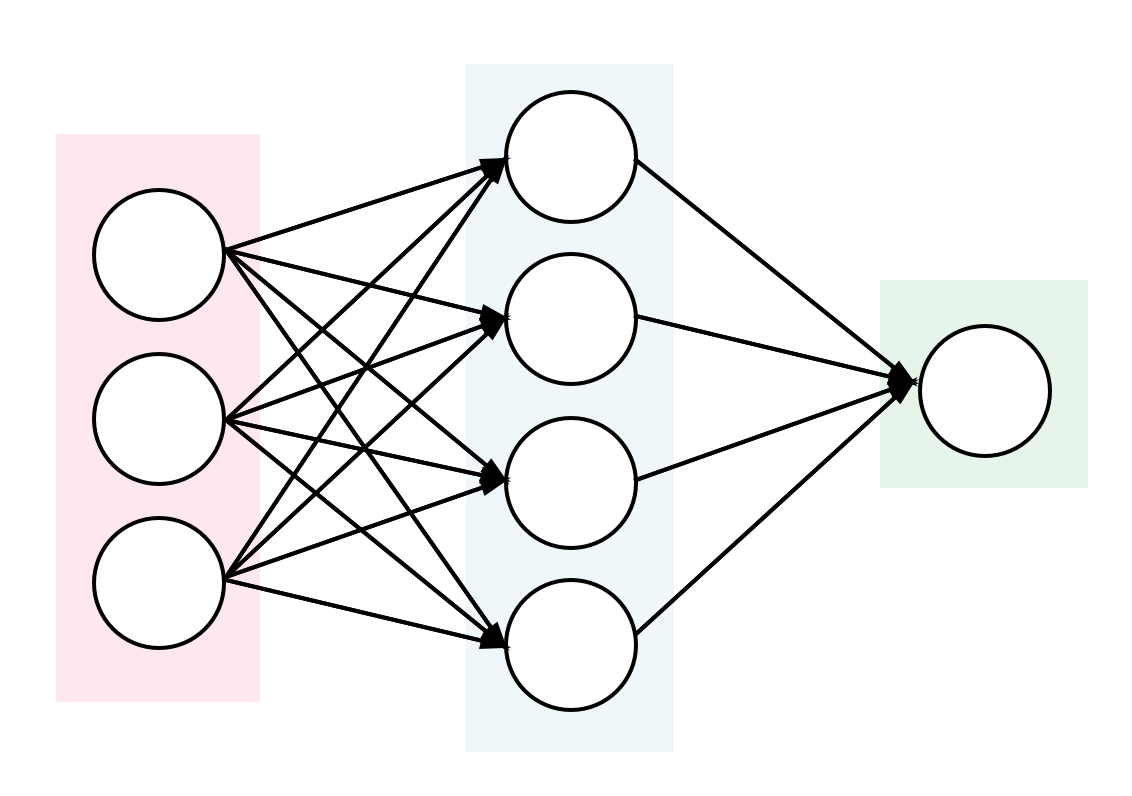
\includegraphics[width=5cm]{images/nn.png}}

\Put(0, -75){input $x$}
\Put(45, -85){hidden layer}
\Put(135, 35){output $y=f_{w, v}(x)= w \cdot  \sum_j (v_j^\top x)_+ $}
\Put(30, 90){$v_j$}
\Put(35, 125){$j$th neuron}
\Put(75, 75){$w$}

\vspace{6em}


$\min_{w, v} \frac{1}{n} \sum_{i=1}^n \ell \big(f_{w, v}(x_i), y_i \big)$ \hspace{5em}$\min_{f \in \mathcal{F}_1} \frac{1}{n} \sum_{i=1}^n \ell \big(f(x_i), y_i \big)$

\vspace{1em}

non-convex problem \hspace{1.5em} {\LARGE $\rightarrow$} \hspace{1em} convex... but infinite-dimensional


\end{frame}


\subsection{Regularized convex problem}

\begin{frame}{\subsecname}

\textit{Variation norm} of $f$: $\gamma_1(f)=||w||_1$ if finite number of neurons.

extends to any number of neurons using Radon measures.

$$\min_{\gamma_1(f) < \delta}  \frac{1}{n} \sum_{i=1}^n \ell \big(f(x_i), y_i \big)$$

\vspace{1em}

\textit{Generalization results}:

\begin{itemize}

\item $f$ decomposed with at most $O(\gamma_1(f)^2/\varepsilon^2)$ neurons with error $\varepsilon$

\item $\mathcal{F}_1$ contains non-smooth functions

\item convex neural networks are adaptive to structure

\end{itemize}

\hspace{3em}$\rightarrow$ \textit{breaking the curse of dimensionality}





\end{frame}


\section{Optimization}


\subsection{Optimizing with Frank-Wolfe}

\begin{frame}{\subsecname}



\textit{How to solve a constrained problem in high-dimension?}

$$\min_{\gamma_1(f) < \delta}  \frac{1}{n} \sum_{i=1}^n \ell \big(f(x_i), y_i \big)$$

\vspace{2em}

Frank-Wolfe algorithm: incrementally add neurons.

\begin{itemize}

\item convergence rate $O(1/t)$ after $t$ steps

\item but each step requires to add a new neuron

\item and this is NP-hard!

\end{itemize}

\end{frame}

\subsection{Optimizing with Gradient Descent}

\begin{frame}{\subsecname}


Neural network as a mixture of particles $v$ with weight $w$

In the space of measures: $\mu = \sum_j w_j \delta_{v_j}$

\vspace{1.5em}


\Put(195, -220){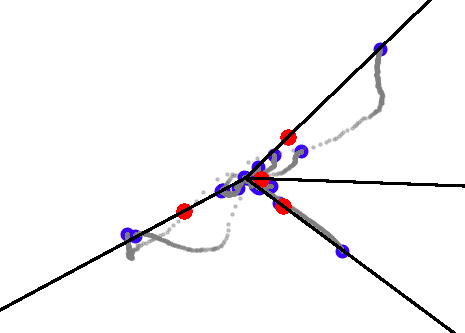
\includegraphics[width=4.5cm]{images/relu.png}}


Result from optimal transport using Wasserstein gradient flow:

\begin{itemize}
\item assumptions on \textit{homogeneity} and \textit{initialization}

\item infinite particle limit

\item continuous time limit
\end{itemize}
\hspace{2em} $\rightarrow$ Convergence to a \textit{global} minimum



\end{frame}

\section{Experiments}

\begin{frame}{\secname}

How much overparametrization is needed for global convergence?

\begin{center}

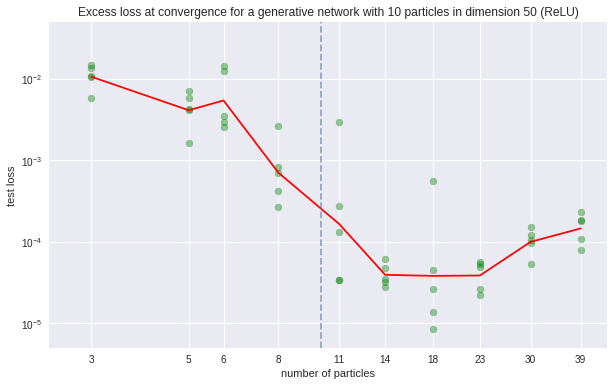
\includegraphics[width=8cm]{images/lossr.png}

\end{center}
%Influence of the initialization?

\end{frame}

\begin{frame}{\secname}

Influence of the initialization?

\vspace{1em}


\hspace{1em} 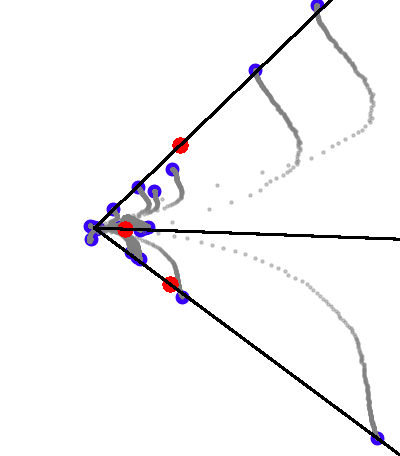
\includegraphics[height=4cm]{images/005.png} \hspace{2em}
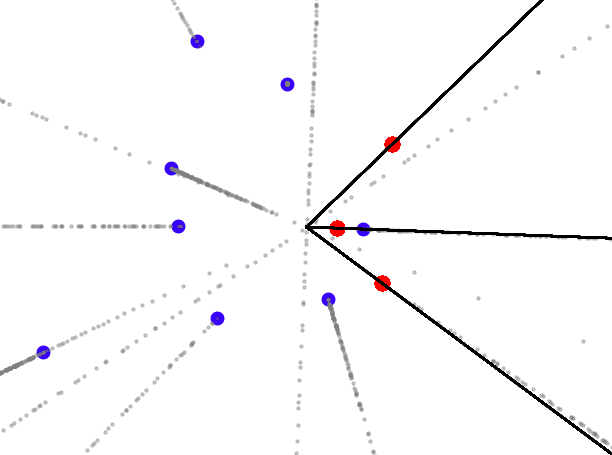
\includegraphics[height=4cm]{images/10.png}
\begin{center}

 \hspace{4em} $r_0 = 0.05$  \hspace{9em} $r_0=10$ \hspace{5em} 

Initial norm of each particle $r_0$
\end{center}

\end{frame}

\section{Conclusion \& Perspectives}

\begin{frame}{\secname}

A novel way to understand the convergence of neural networks;

linking the original non-convex problem to the space of \textit{measures}, hence to optimal transport.

\vspace{1em}

Studying gradient descent through \textit{gradient flows} is promising.

\vspace{1em}

$\rightarrow$ How far from practical applications is this \textit{ideal} dynamics?
\begin{itemize}
\item link between overparametrization and dimension
\item iterative algorithm as a continuous time process
\item practical rules to initialize neural networks
\end{itemize}

\end{frame}

\subsection{References}

\begin{frame}{\subsecname}

\begin{itemize}

\item Bengio, Y., Roux, N.~L., Vincent, P., Delalleau, O., and Marcotte, P. (2006). Convex neural networks. In \textit{Advances in neural information processing systems}

\item Bach, F. (2017). Breaking the curse of dimensionality with convex neural networks. In \textit{Journal of Machine Learning Research}

\item Chizat, L. and Bach, F. (2018).
On the global convergence of gradient descent for over-parameterized
  models using optimal transport. In \textit{Advances in neural information processing systems}
\end{itemize}

\end{frame}
\end{document}
